% Define document class
\documentclass[twocolumn]{aastex631}


\usepackage{listings}

\lstdefinestyle{bash}{%
    language=bash,
    basicstyle=\ttfamily\footnotesize,
    texcsstyle=*\bf\color{black},
    numbers=none,
    breaklines=true,
    commentstyle=\color{red},
    frame=single
}
\lstdefinestyle{LaTeX}{%
    language=[LaTeX]TeX,
    basicstyle=\ttfamily\footnotesize,
    texcsstyle=*\bf\color{black},
    numbers=none,
    breaklines=true,
    commentstyle=\color{red},
    frame=single,
    tabsize=2,
    keywords={begin,caption,label,end,includegraphics},   
}
\definecolor{lsthilite}{rgb}{0.0,0.0,1.0}

% Begin!
\begin{document}

% Title
\title{\showyourwork: a workflow for open source scientific articles}

% Author list
\author[0000-0002-0296-3826]{Rodrigo Luger}

% Abstract with filler text
\begin{abstract}
    Abstract coming soon.
\end{abstract}

% Main body with filler text
\section{Introduction}

Introduction coming soon.

\section{Repository structure}

\begin{figure}[ht!]
    \begin{centering}
        \includegraphics[width=0.5\linewidth]{figures/tree.pdf}
        \caption{
            Basic repository structure for an open source scientfic article.
        }
        \label{fig:tree}
    \end{centering}
\end{figure}

See Figure~\ref{fig:tree}.

\section{Automatic figure generation}

\showyourwork determines the relationship between a figure (e.g., a \texttt{*.pdf} image) and the script that generated it (e.g., a \texttt{*.py} file) via inspection of the \texttt{figure} environment in the \texttt{TeX} file. 
Specifically, it inspects the \texttt{{\textbackslash}includegraphics} and \texttt{{\textbackslash}label} commands to infer the name of the figure and the script that generated it, respectively.
Consider the following snippet, used to generate Figure~\ref{fig:eccentricity}:
%
\begin{lstlisting}[
    style=LaTeX,
    otherkeywords={figures/eccentricity.pdf,fig:eccentricity},
    emph={figures/eccentricity.pdf,fig:eccentricity},
    emphstyle={\color{lsthilite}}
]
\begin{figure}
  \begin{centering}
    \includegraphics{figures/eccentricity.pdf}
    \caption{...}
    \label{fig:eccentricity}
  \end{centering}
\end{figure}
\end{lstlisting}
%
The convention in \showyourwork is to infer the parent script for a figure referenced in an \texttt{includegraphics} call (in this case, {\color{lsthilite}\texttt{figures/eccentricity.pdf}}) from the figure \texttt{label}. 
Specifically, if a label starts with {\color{lsthilite}\texttt{fig:}}, the remainder of the label (e.g., {\color{lsthilite}\texttt{eccentricity}}) is interpreted as the name of a script in the \texttt{figures/} directory which can be executed to produce that figure. 
By default, figure scripts are expected to be \texttt{Python} scripts, so in this case \showyourwork will attempt to run
%
\begin{lstlisting}[
    style=bash
]
python eccentricity.py
\end{lstlisting}
%
from within the \texttt{figures/} directory to generate \texttt{eccentricity.pdf}.

\begin{figure}[ht!]
    \begin{centering}
        \includegraphics[width=\linewidth]{figures/eccentricity.pdf}
        \caption{
            The effect of eccentricity on the detectability of a \emph{LISA} source; reproduced from Figure 3 in \citet{Wagg2021}.
        }
        \label{fig:eccentricity}
    \end{centering}
\end{figure}

\begin{figure}[ht!]
    \begin{centering}
        \includegraphics[width=\linewidth]{figures/luhman16b.pdf}
        \caption{
            16 \emph{CRIRES} spectra of WISE 1049-5319B spanning a full rotation period of the brown dwarf; adapted from Figure 14 in \citet{Luger2021}. 
            Data originally from \citet{Crossfield2014}.
        }
        \label{fig:luhman16b}
    \end{centering}
\end{figure}

\begin{figure}[ht!]
    \begin{centering}
        \includegraphics[width=\linewidth]{figures/rossbyridge.pdf}
        \caption{
            A pile-up of stars in the rotation period-temperature space at slightly faster rotation than the sun (orange dot); adapted from Figure 1 in David et al. (in prep).
        }
        \label{fig:rossbyridge}
    \end{centering}
\end{figure}

\begin{figure}[ht!]
    \begin{centering}
        \includegraphics[width=\linewidth]{figures/HD118203_transit.pdf}
        \includegraphics[width=\linewidth]{figures/HD118203_corner.pdf}
        \caption{
            The phase-folded transit of HD 118203b in \emph{TESS} (\emph{top}) and the inferred joint posterior distributions over its period, radius, and impact parameter (\emph{bottom}); adapted from the \texttt{exoplanet} documentation \citep{ForemanMackey2021}.
            Both figures were generated from the same \texttt{Python} script in the \texttt{src/figures} directory (linked to in the \texttt{GitHub} icon in the margin). The other margin icon indicates that these figures depend on a dataset (a \texttt{.npz} file containing the posterior samples), which is automatically generated by \showyourwork and uploaded to Zenodo. 
            Users wishing to reproduce the results in this paper can choose whether to re-generate this dataset or download a static version from Zenodo (linked to in the margin).
        }
        \label{fig:HD118203}
    \end{centering}
\end{figure}

\begin{figure}[ht!]
    \begin{centering}
        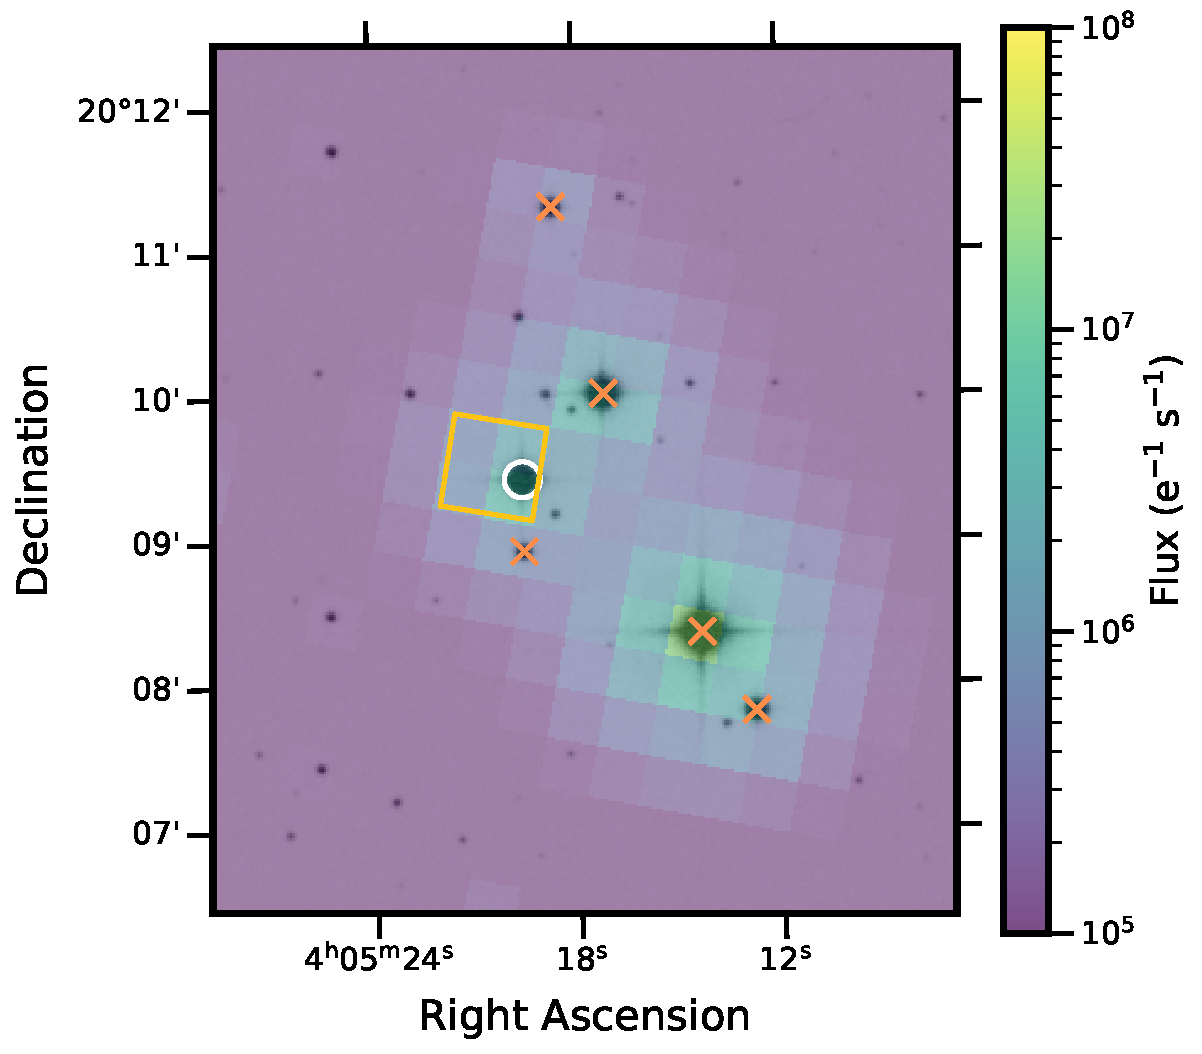
\includegraphics[width=\linewidth]{static/TESSaperture.pdf}
        \caption{
            \emph{TESS} target pixel file (TPF) of V1298 Tau
            overlaid with an r-band sky image from the Digitized Sky Survey (DSS);
            reproduced from Figure 1 in \citet{Feinstein2021}.
            This figure exists as a static PDF, with no associated script to
            generate it.
            We therefore include it in the \texttt{src/static} directory, which tells \showyourwork to not attempt to generate it. 
            By default, margin icons are not added to static figures.
            Here we manually add an icon linking to the original paper using the \texttt{\textbackslash marginicon} command.
        }
        \marginicon{%
            \href{https://ui.adsabs.harvard.edu/abs/2021arXiv211108660F}{\color{sywBlue}\faNewspaper[regular]}
        }
        \label{fig:eclipse}
    \end{centering}
\end{figure}

\begin{figure*}[ht!]
    \begin{centering}
        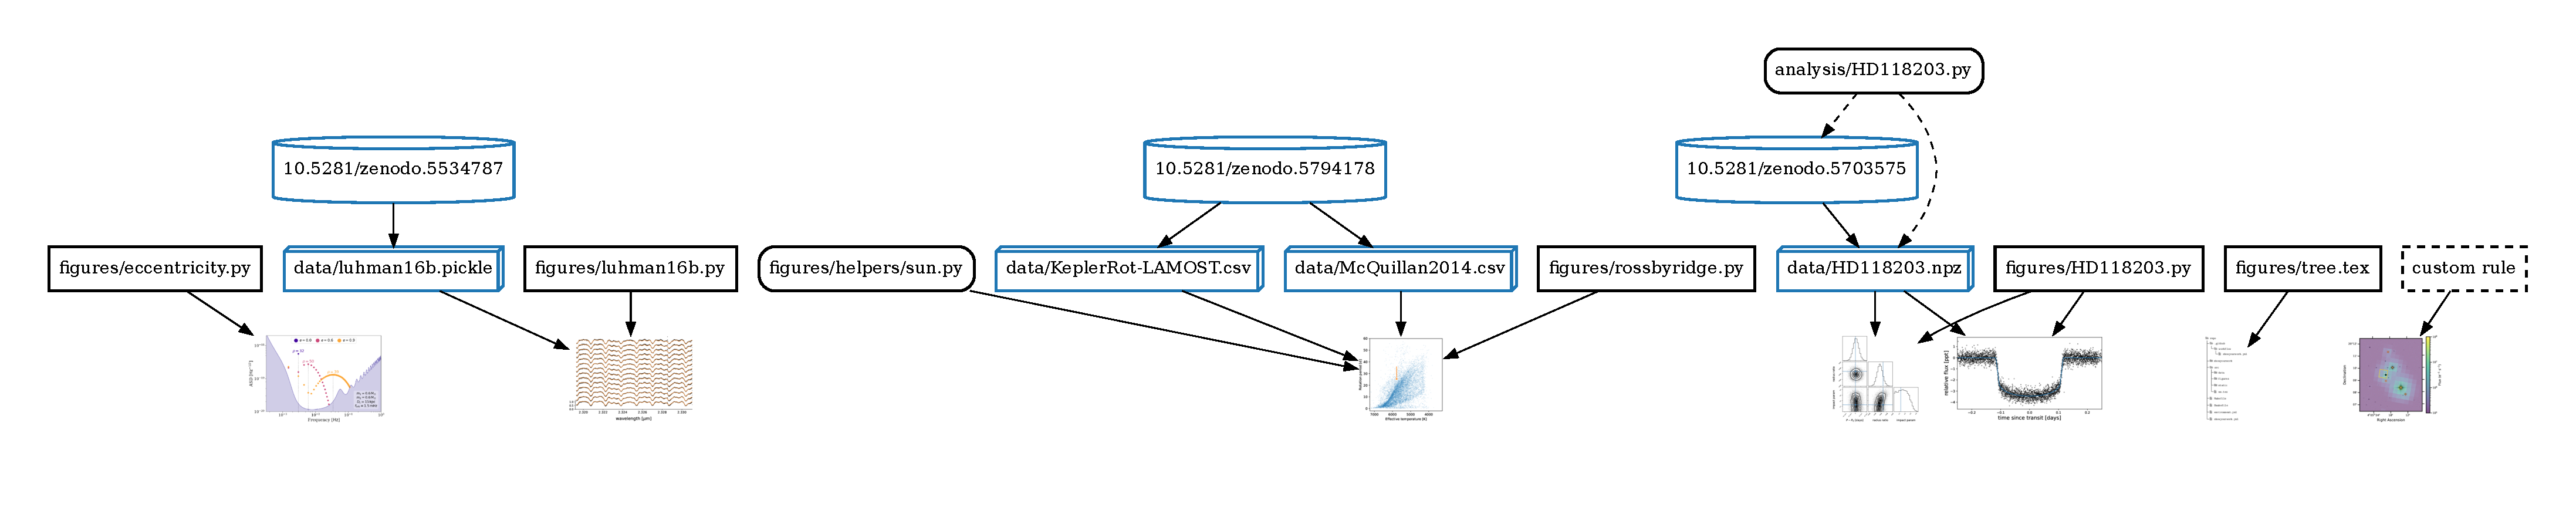
\includegraphics[width=\linewidth]{figures/dag.pdf}
        \caption{
            A directed acyclic graph (DAG) showing the build process for each of the (other) figures in this article. 
            Figure scripts are represented by black rectangles; helper scripts (such as ones imported by figure scripts or used in dataset generation) are similar, but have rounded edges.
            Blue cylinders correspond to Zenodo records; blue boxes correspond to datasets.
        }
        \label{fig*:dag}
    \end{centering}
\end{figure*}

\bibliography{bib}

\end{document}
